\begin{homeworkProblem}
    Solve the following difference equations subject to the specified $x$ values and
    sketch the solutions:
    \begin{enumerate}
        \item $x_n - 5x_{n-1} + 6x_{n-2} = 0;\quad x_0 = 2, x_1 = 5.$
        \addtocounter{enumi}{1}
        \item $x_n - x_{n-2} = 0;\quad x_1 = 3, x_2 = 5.$
        \addtocounter{enumi}{1}
        \item $x_{n+2} + x_{n+1} - 2x_n = 0; \quad x_0 = 6, x_1 = 3.$
    \end{enumerate}
    
    \segline
    
    \solution
    
    \begin{enumerate}
        \item The characterictic function is \[
            \lambda^2 - 5\lambda + 6 = 0
        \]
        The characterictic roots are \[
            \lambda_1 = 2, \quad \lambda_2 = 3.
        \]
        The general solution should be \[
            A_1 2^n + A_2 3^n  = 0.
        \]
        Plug in $x_0 = 2$ and $x_1 = 5$, we have \[
            \left\{
            \begin{aligned}
                &A_1 + A_2  = 2\\
                &2A_1  + 3A_2 = 5
            \end{aligned}
            \right.
            \quad
            \Rightarrow
            \quad
            \left\{
            \begin{aligned}
                A_1 = 1\\
                A_2 = 1
            \end{aligned}
            \right.
        \]
        To sum up, the specific solution should be $$
            x_n = 2^n + 3^n.
        $$
        And the plot would look like
        \begin{figure}[H]
            \centering
            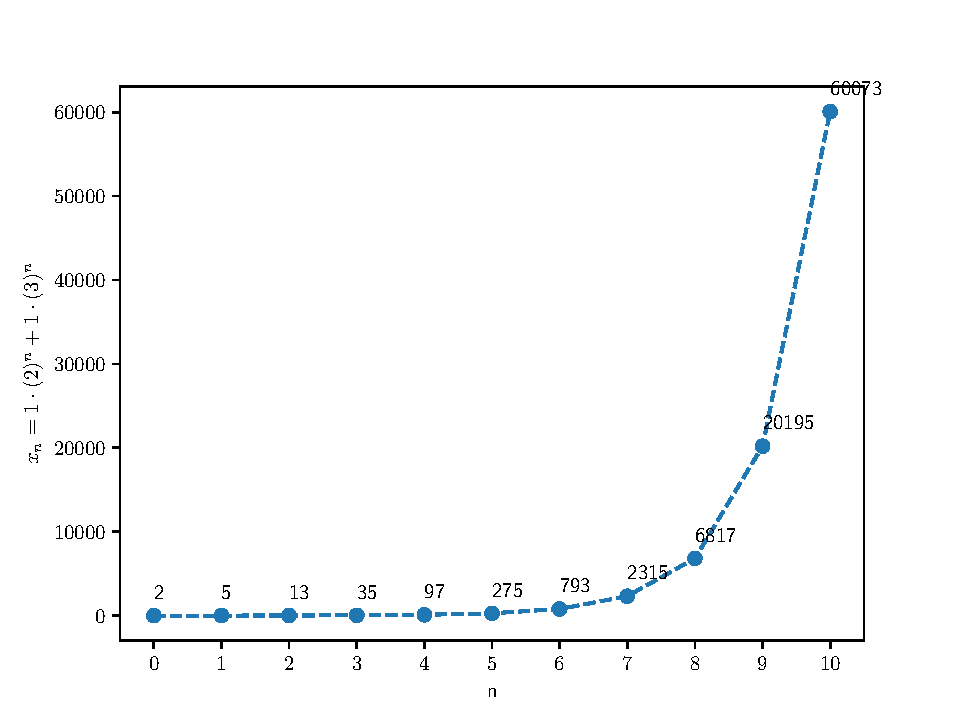
\includegraphics[scale=0.5]{fig/fig2(a).pdf}
        \end{figure}
        \addtocounter{enumi}{1}
    
        \item The characterictic function is \[
            \lambda^2 - 1 = 0
        \]
        The characterictic roots are \[
            \lambda_1 = -1, \quad \lambda_2 = 1.
        \]
        The general solution should be \[
            A_1 (-1)^n + A_2  = 0
        \]
        Plug in $x_1 = 3$ and $x_2 = 5$, we have \[
            \left\{
            \begin{aligned}
                &-A_1 + A_2  = 3\\
                &A_1  + A_2 = 5
            \end{aligned}
            \right.
            \quad
            \Rightarrow
            \quad
            \left\{
            \begin{aligned}
                A_1 = 1\\
                A_2 = 4
            \end{aligned}
            \right.
        \]
        To sum up, the specific solution should be $$
            x_n = (-1)^n + 4.
        $$
        And the plot would look like
        \begin{figure}[H]
            \centering
            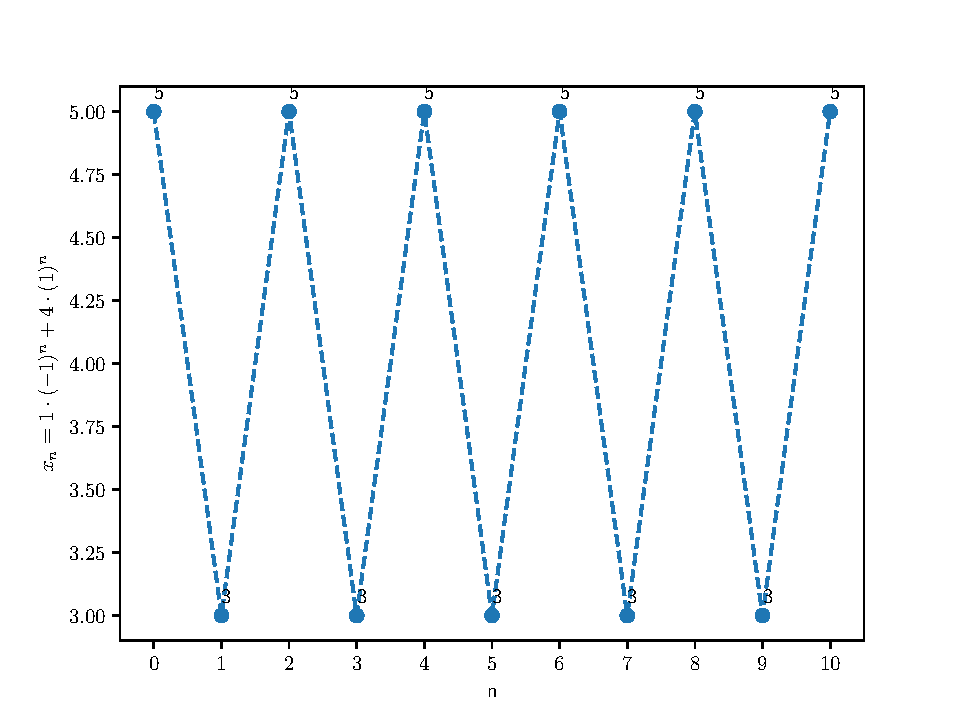
\includegraphics[scale=0.5]{fig/fig2(c).pdf}
        \end{figure}
        \addtocounter{enumi}{1}
    \pagebreak
        \item The characterictic function is \[
            \lambda^2 + \lambda -2 = 0
        \]
        The characterictic roots are \[
            \lambda_1 = 1, \quad \lambda_2 = -2.
        \]
        The general solution should be \[
            A_1 + A_2 (-2)^n = 0
        \]
        Plug in $x_0 = 6$ and $x_1 = 3$, we have \[
            \left\{
            \begin{aligned}
                &A_1 + A_2  = 6\\
                &A_1 - 2A_2 = 3
            \end{aligned}
            \right.
            \quad
            \Rightarrow
            \quad
            \left\{
            \begin{aligned}
                A_1 = 5\\
                A_2 = 1
            \end{aligned}
            \right.
        \]
        To sum up, the specific solution should be $$
            x_n = (-2)^n + 5.
        $$
        And the plot would look like
        \begin{figure}[H]
            \centering
            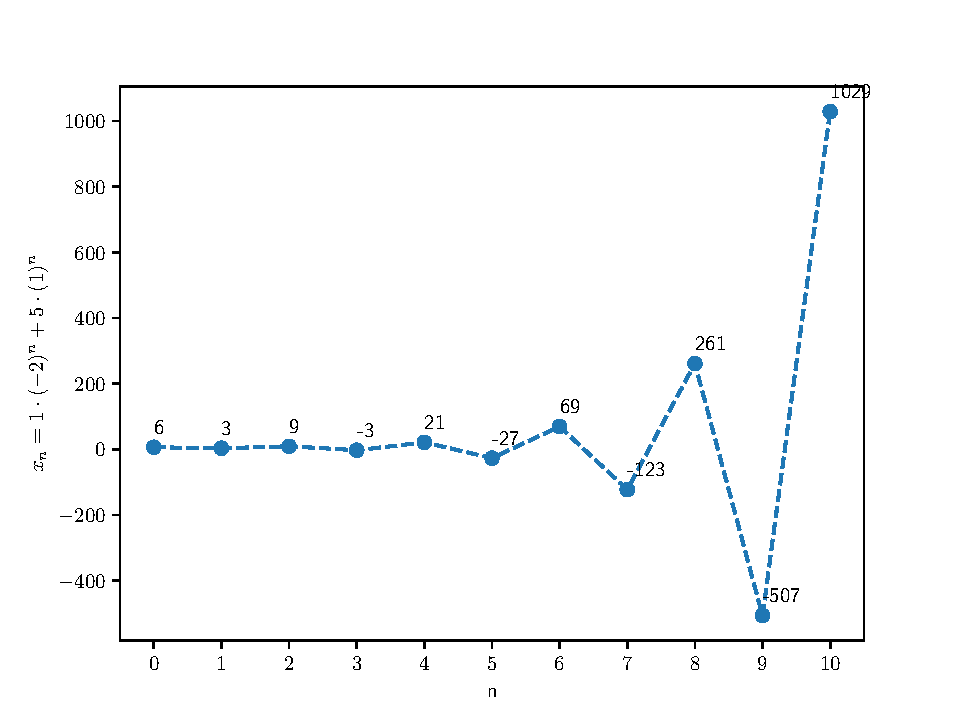
\includegraphics[scale=0.5]{fig/fig2(e).pdf}
        \end{figure}
    \end{enumerate}
    
    \end{homeworkProblem}
    